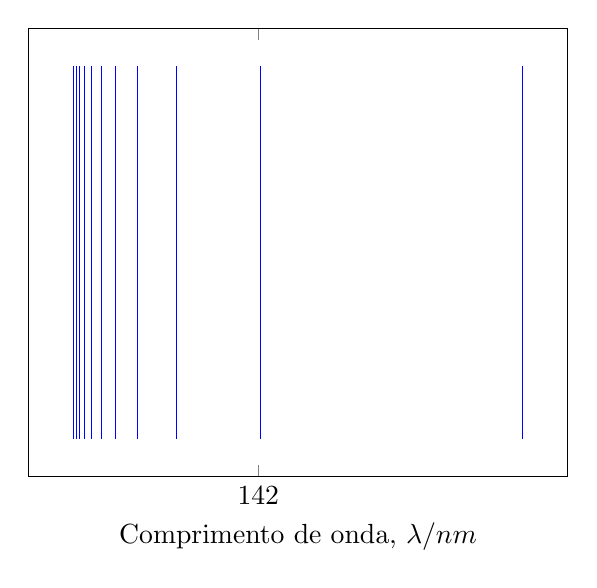
\begin{tikzpicture}
    \begin{axis}
        [
            domain = 0:2700,
            xlabel = {Comprimento de onda, $\lambda/\unit{nm}$},
            xtick = {142}, 
            ytick=\empty,
        ]
    \pgfplotsinvokeforeach { 4, 5, 6, 7, 8, 9, 10, 11, 12, 13, 14 }
        {
            \addplot[blue] coordinates
            {
                ( (1240/13.6)/(1-9/#1^2), 0 )
                ( (1240/13.6)/(1-9/#1^2), 1 )
            };
        }
\end{axis}
\end{tikzpicture}
